%!TEX root = /Users/simo/Documents/PFC/Chapter3/chapter3.tex
\section{Primer ciclo} % (fold)
\label{sec:primer_ciclo}
La metodología de desarrollo ágil defiende un desarrollo iterativo, por ciclos pequeños que generen de forma rápida ciertas funcionalidades. Cada ciclo amplia funcionalidades hasta que al final estén todas incluidas. Cada ciclo debe ser completo, con sus fases de análisis de requisitos, diseño, implementación y revisión. La fase de documentación tiene como resultado este capítulo.

En este primer ciclo, se pretende obtener todas las funcionalidades necesarias para poder crear y editar documentos.

\subsection{Análisis de requisitos} % (fold)
\label{sub:análisis_de_requisitos}

Gracias a que se ha tratado la implementación del Javascript de forma previa a este ciclo, se conocen ya los requisitos básicos necesarios para poder utilizar el motor de dibujo. De forma detallada, las funcionalidades requeridas para este ciclo son las siguientes:

\begin{itemize}
  \item Poder crear, editar y borrar documentos, dándoles un título, una descripción y asignándole una cantidad de páginas fija, mediante interacción normal por HTML.
  \item Tener soporte para documentos, páginas y los elementos contenidas en ellas, de forma que el motor de comunicación en Javascript pueda comunicarse con la aplicación para editar las pizarras.
\end{itemize}

% subsection análisis_de_requisitos (end)

\subsection{Diseño} % (fold)
\label{sub:diseño}

El primer paso natural a la hora de planear un ciclo en Ruby on Rails es planeando la estructura de la aplicación en cuanto a modelos y controladores se refiere. Los modelos serán necesarios para poder guardar los datos en la base de datos, y deben estar relacionados adecuadamente de forma que sea fácil y directo acceder a datos de modelos \emph{cercanos}. También es importante considerar los controladores en los que agrupar las funciones. Sería posible implementar la aplicación entera en un controlador enorme, pero obviamente esto no sería práctico ni productivo.

\subsubsection{Modelos} % (fold)
\label{ssub:modelos}

El diagrama de clases es extremadamente sencillo en este ciclo. Solamente son necesarias tres clases, una para representar el documento, otra para las páginas y otra para los elementos. Durante la discusión sobre la implementación del javascript ya se discutió que la descripción de cada elemento se guardaría como una cadena de texto JSON representativa de los elementos que se crean mediante javascript, por lo tanto, un elemento no necesita más variedad de atributos.

El diagrama final puede observarse en la figura \ref{fig:uml1}

\begin{figure}[h!]
\centering
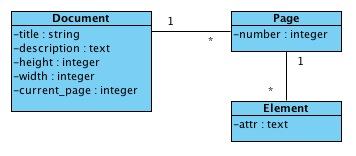
\includegraphics{uml1.png}
\caption{Clases del dominio, 1er ciclo}\label{fig:uml1}
\end{figure}


% subsubsection modelos (end)

\subsubsection{Controladores} % (fold)
\label{ssub:controladores}

En estos momentos se considera suficiente agrupar todas las funcionalidades que traten con los documentos dentro de un solo controlador, \texttt{documents\_controller}. 

% subsubsection controladores (end)

% subsection diseño (end)

\subsection{Implementación} % (fold)
\label{sub:implementacion}

Para inicializar una aplicación en rails, hay que crear dicha aplicación, y configurar la conexión con la base de datos. Desde el principio, se le ha dado el nombre \texttt{drawme}. 

\begin{verbatim}
rails drawme
\end{verbatim}

\subsubsection{Modelos} % (fold)
\label{ssub:modelos}

Este comando generará los archivos que formen el esqueleto de la aplicación. Una vez hecho esto, hay que generar los modelos que se han planeado:

\begin{verbatim}
  $ script/generate model Document
  $ script/generate model Page
  $ script/generate model Element
\end{verbatim}

Estos comandos generarán los archivos dentro de la carpeta \texttt{/app/models}, además de las \emph{migraciones} correspondientes para crear las tablas en la base de datos. Una migración es una acción sobre la base de datos, de cualquier tipo. Dentro de la carpeta \texttt{/db/migrations} se encuentran, ordenadas de forma temporal mediante un timestamp. Gracias a esto se pueden ir realizando modificaciones sobre la base de datos de forma ordenada, permitiendo así, por ejemplo, que si en un futuro se pretende realizar una modificación, no se tenga que eliminar la base de datos entera y volverla a crear.

A forma de ejemplo, la migración para la tabla del modelo \texttt{Document} será así:

\begin{verbatim}
  class CreateDocuments < ActiveRecord::Migration
    def self.up
      create_table :documents do |t|
        t.string :title
        t.text :description
        t.integer :current_page, :default => 1
        t.integer :height, :default => 600
        t.integer :width, :default => 800
        t.timestamps
      end
    end

    def self.down
      drop_table :documents
    end
  end
\end{verbatim}

Ya en este punto se pone en práctica el concepto de \emph{convention over configuration}, en que se ha creado el modelo \texttt{Document}, y la migración generada llama a la tabla de la base de datos \texttt{documents}. Esto siempre es así, un modelo es un nombre en singular, y su tabla es el equivalente en plural. Sabiendo esto, no habrá en ningún momento problemas de nomenclatura, y en caso de que sea necesario llamar a una tabla con un nombre distinto al de su modelo, será necesario añadir una línea en su modelo correspondiente (en este caso \texttt{/app/models/document.rb}).

Un documento puede tener múltiples páginas, y según las prácticas habituales para implementar este tipo de relaciones en bases de datos relacionales, hay que añadir una clave externa en la tabla de las páginas. Para hacer esto, en Ruby on Rails se haría lo siguiente:

\begin{verbatim}
  class CreatePages < ActiveRecord::Migration
    def self.up
      create_table :pages do |t|
        t.integer :number, :null => false
        t.references :document
        
        t.timestamps
      end
      add_index :pages, :document_id
    end

    def self.down
      drop_table :pages
    end
  end
\end{verbatim}

Por convención, los campos que referencian otra tabla, tienen la nomenclatura del tipo \texttt{modelo\_id}, y se aprovecha en este caso para añadir un índice sobre este campo, para que cuando sea necesario consultar las páginas de un documento, no sea necesario recorrer la tabla de páginas entera.

La migración para \texttt{Element} es igual a la de \texttt{Page}.

\begin{verbatim}
  class CreateElements < ActiveRecord::Migration
    def self.up
      create_table :elements do |t|
        t.text :attr, :null => false 
        t.references :page

        t.timestamps
      end
      add_index :elements, :page_id
    end

    def self.down
      drop_table :elements
    end
  end
\end{verbatim}

Para trasladar estas migraciones a la base de datos es necesario ejecutar la línea siguiente en la línea de comandos:

\begin{verbatim}
  $ rake db:migrate
\end{verbatim}

Estas migraciones, no obstante, solamente sirven para tratar con la base de datos. Para que la aplicación sepa que un \texttt{Document} tiene múltiples \texttt{Pages}, es necesario dejar constancia en los modelos:

\begin{verbatim}
  class Document < ActiveRecord::Base
    has_many :pages, :dependent => :destroy
    has_many :elements, :through => :pages
  end
\end{verbatim}

\begin{verbatim}
  class Page < ActiveRecord::Base
    has_many :elements, :dependent => :destroy
    belongs_to :document
  end
\end{verbatim}

\begin{verbatim}
  class Element < ActiveRecord::Base
    belongs_to :page
    belongs_to :document, :through => :page
  end
\end{verbatim}


Con estas líneas, será posible en un futuro, ejecutar instrucciones como las siguientes:

\begin{verbatim}
  # Añadir una página a un documento
  document.pages << Page.new  
  
  # Añadir un elemento a una página
  page.elements << Element.create(:attr => "...") 
  
  # Borrar todas las páginas de un documento
  document.pages.clear
\end{verbatim}

Cualquier operación que trate las relaciones entre estos elementos será posible de forma más sencilla, siempre tratando con la base de datos de forma transparente. 

% subsubsection modelos (end)

\subsubsection{Controladores y vistas} % (fold)
\label{ssub:controlador}

De forma similar a los modelos, para generar los archivos necesarios para un controlador:

\begin{verbatim}
  $ script/generate controller Documents
\end{verbatim}

El archivo generado, utilizando las convenciones, será \texttt{/app/controllers/documents\_controller.rb}. Dentro de este archivo, cada función implementada tendrá una traducción directa en las capa de vistas, por lo tanto el proceso de implementar acciones en controladores suele ir al mismo ritmo que se van implementando las vistas.

Debido a que es el primer ciclo, y que de momento aún no se tiene muy claro cómo acabará estructurándose la web, se optará por tener lo que en Rails se llama un \emph{Scaffold} con unas pocas modificaciones, para poder editar los documentos. Un Scaffold es una envoltura para un modelo, con las cuatro operaciones básicas que se pueden querer realizar: crear, mostrar, modificar y borrar (\texttt{create}, \texttt{show}, \texttt{update} y \texttt{destroy}). Debido a la naturaleza de la web, es necesario otras acciones, previas a estas cuatro. Por ejemplo, antes de crear un documento, es necesario mostrar un formulario en el que rellenar los datos necesarios. Dicha acción se llamaría \texttt{new}. Para poder mostrar un elemento en concreto, primero hay que listar los que hay, y dicha acción se llama \texttt{index}. Para poder modificar un elemento primero hay que mostrar como está en este instante, además de proporcionar un formulario con el que poder especificar los cambios. Ésta acción se llamaría \texttt{edit}. Para eliminar un elemento solo es necesario saber qué elemento eliminar, por lo tanto es posible ejecutar tanto desde \texttt{show} como desde \texttt{index}.

Éstas cuatro acciones forman el llamado \texttt{CRUD} (Create, Retrieve, Update y Delete), y equivalen a las cuatro comentadas, que junto con las otras tres, forman las siete acciones básicas de un controlador de Scaffold.

Puesto que estas acciones son tan comunes, Rails proporciona una forma de generar un Scaffold sencillo de forma automática, para utilizar como punto de partida.

\begin{verbatim}
  script/generate scaffold Document
\end{verbatim}

Gracias a las convenciones de Rails, este Scaffold buscará el modelo \texttt{Document} y creará el controlador \texttt{documents\_controller} con el código adecuado, y las vistas correspondientes.

Este scaffolding, sin embargo, no tiene en cuenta las relaciones entre modelos, ni ningún comportamiento personalizado que se quiera tener. Así, los cambios necesarios para adecuar este scaffold al gusto de la aplicación serían los siguientes:

\begin{itemize}
  \item En el momento de crear un documento, añadirle un número fijo de páginas vacías, con sus números de páginas correspondientes.
  \item El atributo \texttt{current\_page} no debe ser editable, de momento, puesto que se manejará mediante la interfaz javascript.
\end{itemize}

Con estos pasos se puede considerar la primera funcionalidad objetivo cumplida. La segunda funcionalidad es permitir tratar con la interfaz, mediante la comunicación con ajax y transportando elementos en formato JSON. Las funciones necesarias para ello se pueden resumir en las siguientes:

\begin{description}
  \item[\texttt{add\_element}] recibiendo para qué página (y por consiguiente, qué documento), y el objeto en JSON, y retornando el identificador del mismo una vez guardado.
  \item[\texttt{remove\_element}] recibiendo el identificador del elemento.
  \item[\texttt{list\_elements}] recibiendo la página (y por consiguiente, el documento), devolviendo el listado de elementos en formato JSON.
  \item[\texttt{change\_page}] recibiendo la página a la que se quiere cambiar.
\end{description}

Cabe destacar de la implementación de estas funciones, la facilidad que da Rails para tratar con peticiones en Ajax. En el caso de la función \texttt{list\_elements}, por ejemplo, lo lógico sería realizar una búsqueda en la base de datos, teniendo luego un vector de elementos, que luego se deberían traducir a JSON, y mostrarse en la vista.

\begin{verbatim}
  def list_elements
    render :json => Page.find(params[:page_id]).elements
  end
\end{verbatim}

Debido a que JSON se ha convertido en un formato standard en este tipo de acciones, Rails usa las librerías de Ruby para la conversión de objetos a sus equivalentes en JSON, y mediante una sola línea es posible devolver un objeto exactamente equivalente al que se tiene en ese momento en Ruby, pero que javascript podrá entender.

Con esto, se tienen las dos funcionalidades originales, y ya sería posible empezar a dibujar en la interficie en Javascript, con múltiples usuarios al mismo tiempo con persistencia en una base de datos.

% subsubsection controlador (end)

% subsection implementacion (end)
% section primer_ciclo (end)